\begin{frame}{Background}
\begin{itemize}
    \item The British railway industry employed 2.5\% of the entire population in 1900.

    \item By 1870 railway networks covered most areas of the UK.
    
    \item The unionization movement in the UK started in 1871.

    \

    \item Mass unionization occurred in the initial year, and slowly grew.
    
    The union group (ASRS) included members from a diverse set of occupations.

    \

    \item Other union groups emerged in the 1880s, impeding the growth of ASRS.
    The other union groups restricted members to specific occupations (Locomotive Engineers, Signalmens, etc).
\end{itemize}
    
\end{frame}

\begin{frame}{Map}
    \begin{figure}
        \centering
        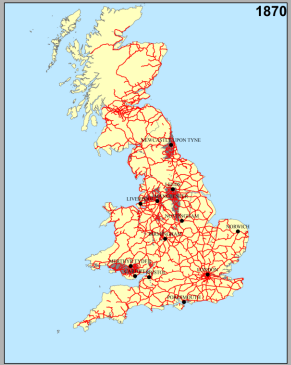
\includegraphics[width = 0.6\textwidth]{Background/Map.png}
        \label{fig:enter-label}
    \end{figure}
\end{frame}

\begin{frame}{Background: Unionization movement}
    \begin{itemize}
        \item 
    \end{itemize}
\end{frame}